%!TEX root = /Users/ego/Boulot/TKZ/tkz-euclide/doc_fr/TKZdoc-euclide-main.tex

\section{Les droites}

Il est bien sûr essentiel de tracer des droites, mais avant il faut pouvoir définir certaines droites particulières comme des médiatrices, des bissectrices, des parallèles ou encore des perpendiculaires. Le principe consiste à déterminer deux points de la droite. 
   

\subsection{Définition de droites}

\begin{NewMacroBox}{tkzDefLine}{\oarg{local options}\parg{pt1,pt2} ou \parg{pt1,pt2,pt3}}
\noindent\emph{L' argument est une liste de deux  ou trois points.    Suivant les cas, la macro définit un ou deux points nécessaires pour obtenir la droite cherchée. Il faut utiliser soit la macro \tkzcname{tkzGetPoint}, soit la macro \tkzcname{tkzGetPoints}.}
  

\medskip
\begin{tabular}{lll}
\toprule
options             & défaut & définition                         \\ 
\midrule
\TOline{mediator}{}{médiatrice. Deux points sont définis} 
\TOline{perpendicular=through\ldots}{}{perpendiculaire à une droite passant par un point} 
\TOline{orthogonal=through\ldots}{}{voir ci-dessus }
\TOline{parallel=through\ldots}{}{parallèle à une droite passant par un point}
\TOline{bisector}{}{bissectrice d'un angle défini par trois points}
\TOline{bisector out}{}{bissectrice extérieure}
\TOline{K}{1}{Coefficient  pour la droite perpendiculaire}
 \bottomrule
\end{tabular}
\end{NewMacroBox}  

\subsubsection{Exemple avec \tkzname{mediator}}  
\begin{tkzexample}[latex=5 cm]
\begin{tikzpicture}[rotate=25]
  \tkzInit
  \tkzDefPoints{-2/0/A,1/2/B}
  \tkzDefLine[mediator](A,B)          \tkzGetPoints{C}{D}
  \tkzDefPointWith[linear,K=.75](C,D) \tkzGetPoint{D}
  \tkzDefMidPoint(A,B)                \tkzGetPoint{I}
  \tkzFillPolygon[color=orange!30](A,C,B,D)
  \tkzDrawSegments(A,B C,D)
  \tkzMarkRightAngle(B,I,C) 
  \tkzDrawSegments(D,B D,A)
  \tkzDrawSegments(C,B C,A)
\end{tikzpicture}
\end{tkzexample}  

\subsubsection{Exemple avec \tkzname{orthogonal} et \tkzname{parallel}}    
\begin{tkzexample}[latex=5 cm]
\begin{tikzpicture}
   \tkzDefPoints{-1.5/-0.25/A,1/-0.75/B,-0.7/1/C}
   \tkzDrawLine[end   = $(d_1)$](A,B)
   \tkzDrawPoints(A,B,C)
   \tkzDefLine[orthogonal=through C](B,A) \tkzGetPoint{c}
   \tkzDrawLine[end   = $(\delta)$](C,c)
   \tkzInterLL(A,B)(C,c) \tkzGetPoint{I}
   \tkzMarkRightAngle(C,I,B) 
   \tkzDefLine[parallel=through C](A,B) \tkzGetPoint{c'}
   \tkzDrawLine[end   = $(d_2)$](C,c') 
   \tkzMarkRightAngle(I,C,c')   
\end{tikzpicture}
\end{tkzexample}

\subsection{Tracer une droite}

Pour tracer une droite, il suffit de donner les deux points et d'utiliser l'option \tkzname{add}. Cette option est due à Mark Wibrow 

\begin{tkzltxexample}[]
  \tikzset{%
    add/.style args={#1 and #2}{
        to path={%
 ($(\tikztostart)!-#1!(\tikztotarget)$)--($(\tikztotarget)!-#2!(\tikztostart)$)%
  \tikztonodes}}}
\end{tkzltxexample}
  
  Cela permet de tracer une partie d'une droite définie par deux points. On utilise pour cela deux valeurs, qui sont des pourcentages par rapport à la longueur du segment défini par les deux points.
  
\begin{tkzexample}[]
\begin{tikzpicture}
   \tkzDefPoints{0/0/A,5/0/B}
   \tkzDrawLine[color=blue,thin, add=1 and 1,end   = $(\delta)$](A,B) 
   \tkzDrawLine[color=red,thick, add=.5 and .5](A,B)
   \tkzDrawPoints(A,B)  \tkzLabelPoints(A,B)
    \tkzDrawLine[color=Maroon,line width=2pt, add=-.2 and -.2 ](A,B)  
  \end{tikzpicture} 
\end{tkzexample} 

 \begin{NewMacroBox}{tkzDrawLine}{\oarg{local options}\parg{pt1,pt2}}
\emph{Les arguments sont une liste de deux points.}

\begin{tabular}{lll}
\toprule
options             & défaut & définition                         \\ 
\midrule
\TOline{add= nb1 and nb2}{.2 and .2}{Permet de prolonger le segment} 
 \bottomrule
\end{tabular}

\medskip 
\emph{\tkzname{add} permet de définir la longueur du trait passant par les points pt1 et pt2. Les deux nombres sont des pourcentages. Les styles de \TIKZ\ sont accessibles pour les tracés}
\end{NewMacroBox}

\subsubsection{Exemple de tracer de droite avec \tkzname{add}}

\begin{tkzexample}[latex=5cm]
\begin{tikzpicture}
 \tkzInit[xmin=-2,xmax=3,ymin=-2.25,ymax=2.25]
 \tkzClip[space=.25]
 \tkzDefPoint(0,0){A} \tkzDefPoint(2,0.5){B}
 \tkzDefPoint(0,-1){C}\tkzDefPoint(2,-0.5){D} 
 \tkzDefPoint(0,1){E} \tkzDefPoint(2,1.5){F} 
 \tkzDefPoint(0,-2){G} \tkzDefPoint(2,-1.5){H}
  \tkzDrawLine(A,B)    \tkzDrawLine[add = 0 and .5](C,D) 
 \tkzDrawLine[add = 1 and 0](E,F)
  \tkzDrawLine[add = 0 and 0](G,H) 
 \tkzDrawPoints(A,B,C,D,E,F,G,H)    
 \tkzLabelPoints(A,B,C,D,E,F,G,H)  
\end{tikzpicture}
\end{tkzexample} 

\newpage
Il est possible de tracer plusieurs droites, mais avec les mêmes options.
\begin{NewMacroBox}{tkzDrawLines}{\oarg{local options}\parg{pt1,pt2 pt3,pt4 ...}}
\emph{Les arguments sont une liste de couples de deux points séparés par des espaces. Les styles de \TIKZ\ sont accessibles pour les tracés.}
\end{NewMacroBox}      

\subsubsection{Exemple avec \tkzcname{tkzDrawLines}}    
\begin{center}
\begin{tkzexample}[latex=7cm]
\begin{tikzpicture}
  \tkzDefPoint(0,0){A}
  \tkzDefPoint(2,0){B}
  \tkzDefPoint(1,2){C}
  \tkzDefPoint(3,2){D}   
  \tkzDrawLines(A,B C,D A,C B,D)
  \tkzLabelPoints(A,B,C,D)
\end{tikzpicture}
\end{tkzexample}
\end{center} 
 
\begin{center}
\begin{tkzexample}[vbox] 
\begin{tikzpicture}
 \tkzInit[xmin=-3,xmax=6, ymin=-1,ymax=6]
 \tkzClip
 \tkzDefPoint(0,0){O}
 \tkzDefPoint(3,1){I}
 \tkzDefPoint(1,4){J}
 \tkzDefLine[bisector](I,O,J)     \tkzGetPoint{i}   
 \tkzDefLine[bisector out](I,O,J) \tkzGetPoint{j}
 \tkzDrawLines[add = 1 and 1,color=red](O,I O,J) 
 \tkzDrawLines[add = 5 and 5,color=blue](O,i O,j) 
\end{tikzpicture} 
\end{tkzexample}
\end{center} 

\newpage
\subsubsection{Une enveloppe}
D'après une figure d'O. Reboux  avec pst-eucl de D Rodriguez
\begin{center}
\begin{tkzexample}[vbox]
\begin{tikzpicture}[scale=1.25]
  \tkzInit[xmin=-6,ymin=-6,xmax=6,ymax=6]  
  \tkzClip 
  \tkzDefPoint(0,0){O} 
  \tkzDefPoint(132:4){A}
  \tkzDefPoint(5,0){B}
  \foreach \ang in {5,10,...,360}{%
    \tkzDefPoint(\ang:5){M}
    \tkzDefLine[mediator](A,M)
    \tkzDrawLine[color=magenta,add= 4 and 4](tkzFirstPointResult,tkzSecondPointResult)}
\end{tikzpicture}
\end{tkzexample}
\end{center}

\newpage
\subsubsection{Une parabole}
D'après une figure d'O. Reboux  avec pst-eucl de D Rodriguez.
Il n'est pas nécessaire de nommer les deux points qui définissent la médiatrice.

\begin{center}
\begin{tkzexample}[vbox]
\begin{tikzpicture}[scale=1.25]
  \tkzInit[xmin=-6,ymin=-6,xmax=6,ymax=6]  
  \tkzClip 
  \tkzDefPoint(0,0){O} 
  \tkzDefPoint(132:5){A}
  \tkzDefPoint(4,0){B}
  \foreach \ang in {5,10,...,360}{%
    \tkzDefPoint(\ang:4){M}
    \tkzDefLine[mediator](A,M) 
    \tkzDrawLine[color=magenta,
             add= 4 and 4](tkzFirstPointResult,tkzSecondPointResult)}
   \end{tikzpicture}
\end{tkzexample}
\end{center}


\subsection{Ajouter des labels aux  droites \tkzcname{tkzLabelLine}} 

 \begin{NewMacroBox}{tkzLabelLine}{\oarg{local options}\parg{pt1,pt2}\marg{label}}

 \begin{tabular}{lll}
 \toprule
 arguments &  défaut  & définition                 \\ 
 \midrule
 \TAline{label}{}{exemple \tkzcname{tkzLabelLine(A,B)\{$\delta$\}}}
 \bottomrule
 \end{tabular}

\medskip
\begin{tabular}{lll}
\toprule
options             & défaut & définition                         \\ 
\midrule
\TOline{pos}{.5}{pos est une option de \TIKZ\ mais essentielle dans ce cas} 
 \bottomrule
\end{tabular}

\medskip
\emph{En option et en plus de \tkzname{pos}, on peut utiliser tous les styles de \TIKZ\ , en particulier le placement avec \tkzname{above}, \tkzname{right}, \dots}

 \end{NewMacroBox}

\subsubsection{Exemple avec \tkzcname{tkzLabelLine}}
Une option importante est \tkzname{pos}, c'est elle qui permet de placer le label le long de la droite. La valeur de \tkzname{pos} peut être supérieure à 1 ou négative.

\begin{tkzexample}[latex=4cm]
\begin{tikzpicture}
   \tkzInit[ymin=-1,ymax=1.5,xmin=-2,xmax=2.5]
   \tkzDefPoints{0/0/A,3/0/B,1/1/C}
   \tkzDefLine[perpendicular=through C,K=-1](A,B)
   \tkzGetPoint{c}
   \tkzDrawLines(A,B C,c)
   \tkzLabelLine[pos=1.25,blue,right](C,c){$(\delta)$} 
   \tkzLabelLine[pos=-0.25,red,left](C,c){encore $(\delta)$} 
\end{tikzpicture}
\end{tkzexample}


\subsection{Configurer les options pour les lignes \tkzcname{tkzSetUpLine}}
voir  \ref{tkzsetupline}
 
\newpage
\subsection{Montrer les constructions de certaines  lignes \tkzcname{tkzShowLine}}

 \begin{NewMacroBox}{tkzShowLine}{\oarg{local options}\parg{pt1,pt2} ou \parg{pt1,pt2,pt3}}
\emph{Ces constructions concernent les médiatrices, les droites perpendiculaires ou parallèles passant par un point donné et les bissectrices. Les arguments sont donc des listes de deux ou bien de trois points. Plusieurs options permettent l'ajustement des constructions. L'idée de cette macro revient à \tkzimp{Yves Combe}}
  

\medskip 
\begin{tabular}{lll}
\toprule
options             & défaut & définition                         \\ 
\midrule
\TOline{mediator}{mediator}{affiche les constructions d'une médiatrice} 
\TOline{perpendicular}{mediator}{constructions pour une perpendiculaire} 
\TOline{orthogonal}{mediator}{idem}
\TOline{bisector}{mediator}{constructions pour une bissectrice}
\TOline{K}{1}{cercle inscrit dans à un triangle }
\TOline{length}{1}{ en cm, longueur d'un arc}
\TOline{ratio} {.5}{rapport entre les longueurs des arcs}
\TOline{gap}{2}{placement le point de construction}
\TOline{size}{1}{rayon d'un arc (voir bissectrice)}
 \bottomrule
\end{tabular}

\emph{Il faut ajouter bien sûr tous les styles de \TIKZ\ pour les tracés}
\end{NewMacroBox}

\subsubsection{Exemple de \tkzcname{tkzShowLine} et \tkzname{parallel}} 

\begin{tkzexample}[latex=5cm]
\begin{tikzpicture}
    \tkzDefPoints{-1.5/-0.25/A,1/-0.75/B,-1.5/2/C}
    \tkzDrawLine(A,B)
    \tkzDefLine[parallel=through C](A,B)  \tkzGetPoint{c} 
    \tkzShowLine[parallel=through C](A,B)
    \tkzDrawLine(C,c)
    \tkzDrawPoints(A,B,C,c)
\end{tikzpicture}
\end{tkzexample}



\subsubsection{Exemple de \tkzcname{tkzShowLine} et \tkzname{perpendicular}} 

\begin{tkzexample}[latex=6cm]
\begin{tikzpicture}
  \tkzInit[xmin=0,xmax=6,ymin=0,ymax=6]
  \tkzClip
  \tkzDefPoint(0,0){A}
  \tkzDefPoint(3,4){B}  
  \tkzDefPoint(2,4){C}
  \tkzDefLine[perpendicular=through C,%
              K=-.5](A,B)
  \tkzGetPoint{c}
  \tkzDefPointBy[projection=onto A--B](c) 
  \tkzGetPoint{h}
  \tkzMarkRightAngle[fill=lightgray](A,h,C)
  \tkzDrawLines[](A,B C,c)
  \tkzDrawPoints(A,B,C,h,c)
\end{tikzpicture}
\end{tkzexample}

\subsubsection{Exemple de \tkzcname{tkzShowLine} et \tkzname{bisector}} 

\begin{tkzexample}[latex=5.25 cm]
\begin{tikzpicture}
 \tkzInit[xmin=0,xmax=7,ymin=0,ymax=7]
 \tkzClip 
 \tkzDefPoints{0/0/A, 6/2/B, 1/6/C}
 \tkzDrawPolygon(A,B,C)  
 \tkzSetUpCompass[color=brown,line width=.1 pt]
 \tkzDefLine[bisector](B,A,C)  \tkzGetPoint{a}
 \tkzDefLine[bisector](C,B,A)  \tkzGetPoint{b}
 \tkzShowLine[bisector,size=2,gap=3](B,A,C)
 \tkzShowLine[bisector,size=1,gap=3](C,B,A)   
 \tkzInterLL(A,a)(B,b) \tkzGetPoint{I}
 \tkzDefPointBy[projection = onto A--B](I) 
 \tkzDrawCircle[radius,color=red,%
 line width=.2pt](I,tkzPointResult) 
 \tkzDrawSegments[color=Maroon!50](I,tkzPointResult)
 \tkzDrawLines[add=0 and 5,color=Maroon!50](A,a B,b) 
\end{tikzpicture}

\end{tkzexample}

\subsubsection{Exemple de \tkzcname{tkzShowLine} et \tkzname{mediator}} 
\begin{tkzexample}[latex=6 cm]
\begin{tikzpicture}
 \tkzInit[xmax=6,ymax=7]
 \tkzGrid
 \tkzDefPoint(2,2){A} 
 \tkzDefPoint(5,4){B}  
 \tkzDrawPoints(A,B)    
 \tkzShowLine[mediator,color=orange,length=1](A,B)
 \tkzGetPoints{i}{j}
 \tkzLabelPoints[below =3pt](A,B)
 \tkzDrawLines[](A,B i,j) 
\end{tikzpicture}
\end{tkzexample}
\endinput